\documentclass{chi-ext}
% Please be sure that you have the dependencies (i.e., additional LaTeX packages) to compile this example.
% See http://personales.upv.es/luileito/chiext/

%% EXAMPLE BEGIN -- HOW TO OVERRIDE THE DEFAULT COPYRIGHT STRIP -- (July 22, 2013 - Paul Baumann)
 \copyrightinfo{Permission to make digital or hard copies of all or part of this work for personal or classroom use is granted without fee provided that copies are not made or distributed for profit or commercial advantage and that copies bear this notice and the full citation on the first page. Copyrights for components of this work owned by others than ACM must be honored. Abstracting with credit is permitted. To copy otherwise, or republish, to post on servers or to redistribute to lists, requires prior specific permission and/or a fee. Request permissions from permissions@acm.org. \\
 {\emph{CHI'14}}, April 26--May 1, 2014, Toronto, Canada. \\
 Copyright \copyright~2014 ACM ISBN/14/04...\$15.00.
 }
%% EXAMPLE END -- HOW TO OVERRIDE THE DEFAULT COPYRIGHT STRIP -- (July 22, 2013 - Paul Baumann)

\title{Applications of Consumer Hardware to Ubiquitous Home Automation}

\numberofauthors{5}
% Notice how author names are alternately typesetted to appear ordered in 2-column format;
% i.e., the first 4 authors on the first column and the other 4 authors on the second column.
% Actually, it's up to you to strictly adhere to this author notation.
\author{
  \alignauthor{
  	\textbf{Kirsten Koa}\\
  	\email{kkoa@ucsd.edu}
  }\alignauthor{
  	\textbf{Chu Shao}\\
  	\email{chsao@eng.ucsd.edu}
  }
  \vfil
  \alignauthor{
  	\textbf{Derek Huynh}\\
  	\email{dbhuynh@ucsd.edu}
  }\alignauthor{
  	\textbf{Patrick Torbett}\\
  	\email{ptorbett@ucsd.edu}
  }
  \vfil
  \alignauthor{
  	\textbf{Calvin Nguyen}\\
  	\email{cbn004@ucsd.edu}
  }
}

% Paper metadata (use plain text, for PDF inclusion and later re-using, if desired)
\def\plaintitle{Applications of Consumer Hardware to Ubiquitous Home Automation}
\def\plainauthor{Kirsten Koa, Derek Huynh, Calvin Nguyen, Chu Shao, Patrick Torbett}
\def\plainkeywords{automation, arduino, kinect, voice, gesture}
\def\plaingeneralterms{Automation}

\hypersetup{
  % Your metadata go here
  pdftitle={\plaintitle},
  pdfauthor={\plainauthor},  
  pdfkeywords={\plainkeywords},
  pdfsubject={\plaingeneralterms},
  % Quick access to color overriding:
  %citecolor=black,
  %linkcolor=black,
  %menucolor=black,
  %urlcolor=black,
}

\usepackage{graphicx}   % for EPS use the graphics package instead
\usepackage{balance}    % useful for balancing the last columns
\usepackage{bibspacing} % save vertical space in references


\begin{document}
\maketitle

\begin{abstract}
We explore the potential of a Microsoft Kinect sensor and Arduino microcontrollers to provide a home automation system with gesture and voice based controls.
The Microsoft Kinect brought depth-sensing cameras to a mainstream consumer audience and a robust voice recognition application programming interface (API).
This approach of using inexpensive hardware allows us to build a scalable solution that augments homes to provide an increased quality of life to the elderly and the disabled.
Gesture based controls allow for users to send control signals without manipulating a physical object, increasing accessibility of objects and ease of use.
Voice recognition allows for increased multitasking that comes with hands-free manipulation of controls and allows some of the disabled to gain independence.
We present our findings on the advantages and shortcomings of building our hardware solution, Vendos.
\end{abstract}

\keywords{\plainkeywords}

\category{H.5.m}{Information interfaces and presentation (e.g., HCI)}{Miscellaneous}.
\category{H.5.2}{User Interfaces}{Ergonomics, Interaction Styles, Voice I/O}.
\category{J.7}{Computer in other systems}{Consumer products}.


% =============================================================================
\section{Introduction}
% =============================================================================

Home automation became more prominent in the late 20th century with the invention of the microcontroller.
Now with cheaper sensing devices, we believe the next wave of home automation and assisted living is here.
We explore the possibilities of depth sensing cameras and voice control with a popular microcontroller design in our solution, Vendos.

The Microsoft Kinect is an depth sensing camera that is backed by a full featured API that supports skeletal tracking and speech recognition.
Our goal is to use the Kinect to create a rich set of gestures designed for controlling the home and supporting voice control inside a residential space.
Given that the Microsoft Kinect assumes that the user is standing face on to the sensor in a relatively quiet environment, we wanted to evaluate our solution in an active living space.

After reviewing our motivation for creating this project and related works that informed our design, we discuss considerations made in designing a home automation system with Kinect and Arduino.
Future directions for this project and the possible applications of Microsoft's exciting Kinect 2 to our design are also presented.
In order to evaluate our solution, we must keep in mind our target audience, the elderly and disabled, and how any failures or successes in our solution affect their health and independence.

We have settled into a way of doing things around the host that copes with the limitations of our physical devices, Vendos hopes to disrupt this by offering new paradigms of control.

% =============================================================================
\section{Motivation and Related Work}
% =============================================================================
As life expectancy rises\cite{_life}, so does the age of the general population.
More and more families are left worrying about the safety and well-being of their elderly members living alone.
Nursing homes are a normal solution to the care of aging family members.
However, private research shows that the elderly dread the loss of their independence and the thought of being sent to a nursing home\cite{_seniors, _caregiving}.
Of course, family members can allow their senior relatives to continue living independently, but there is still a constant uncertainty of their safety and well-being\cite{_caregiving}.
There are many non-technical alternatives to nursing homes to help seniors keep their independence while not having them live alone.
For example, the John Hopkins School of Nursing's CAPABLE helps low-income seniors by providing them with six therapist visits a month, four nurse visits a month, and a total of \$1,200 for home renovations\cite{_nursing}.
The average cost of the services total to around \$3,000 a month versus the average \$6,700 a month senior living costs in America\cite{_forbes}.

Although this may sound like a large discount, the subsidized cost CAPABLE provides is still a significant amount;
an average cost of \$3000 in addition to the senior's original housing cost.
In addition to that, not all seniors are able to benefit from this program because it is still small and experimental.
Since there is no assistance on a day-to-day basis, seniors with motor problems, such as arthritis, still may be forced to live in a nursing home.
This is a problem because, according to the CDC, 24.3\% of women and 18.7\% of men suffer from arthritis\cite{_cdc} alone.

While there are some assistive devices that seniors can purchase to help relieve motor stress, these devices require replacing existing furniture or appliances and for the user to get up and use them\cite{_assistive}.
For example, people with arthritis have trouble flipping small switches and interacting with small controls\cite{_assistive}.
These people could get a motion-detecting lights system or replace their appliances with ones that have bigger knobs, but that would require them to replace their existing lights and appliances.
Our possible solutions to these problems will be discussed further in this paper.

Ever since the launch of Microsoft's Kinect and the Kinect SDK, researchers and technologically-inclined individuals have been experimenting with the many different ways the Kinect's sensors could be utilized beyond the realm of gaming.
Since then, the Kinect has found its way into both the medical field and nursing homes.
 
For example, the Tiger Place is an independent senior housing facility created by Americare, Inc. and the University of Missouri that utilizes Kinect to monitor seniors in their facilities to help ensure their safety\cite{_kinect}.
Currently, they utilize the Kinect to detect falls, access illness, and contact help when they believe it is necessary\cite{_kinect}.
 
Many hospitals have also seen the value it can bring to its patients by utilizing the Kinect in rehabilitation and monitoring efforts.
The Royal Berkshire Hospital in Reading, England uses Kinect to rehabilitate stroke patients and monitor improvements in their movements by using the gestures feature provided by Kinect\cite{_kinect}.
They have also found that utilizing a tool like Kinect brought enjoyment to the patients and decreased their anxiety levels, which they believed led to a faster recovery\cite{_kinect}.
 
We have presented multiple alternatives and proposed solutions to the independent living of seniors.
However, the solutions proposed still require a significant amount of money or the relocation of the elderly to a specified living community.

Vendos' main goal is to help seniors keep their independence in a cost effective manner.
Vendos strives to help seniors with motor problems perform everyday activities such as turning lights on and off, opening and closing the curtains, controlling the television, and interacting with appliances by providing an intuitive voice and gesture interface (enabled by Microsoft's Kinect) that performs these activities on command. 
It also provides a way for seniors to easily contact multiple people (via voice calling and text messaging) for help in an event on an accident.

% =============================================================================
\section{Vendos (Software)}
% =============================================================================

Our solution, Vendos, allows a user to use a standard Kinect camera and an Arduino board that acts as a centralized hub that facilitates controlling and interacting with several appliances and electronic devices by both gesture activation and voice activation.
To achieve the gesture control, the system keeps track of the user's skeletal model and traces the position of specified joints in relation to other joints and triggers a gesture event when a certain sequence of changes is observed.
To achieve voice control, the makes use of a customized grammar and the built-in Kinect microphone.
When the software signals that either a gesture command or a voice command has been detected, that command will be relayed to the Arduino board that is acting as point of connection between the Kinect and the household appliances and devices;
more details of the Arduino board will be covered later in the paper.
 
For this iteration of the project, we decided to include control over these appliances and technologies:
\begin{itemize}\compresslist
\item 	
Lights
\item
Oven Dial
\item
Television
\item
Computer Music Library
\item
Google Voice
\end{itemize}
 
\subsection{Design Considerations for Gesture and Voice}
 
Inspired by the multitude of preexisting touch devices such as Apple's iPhone and the devices powered by Google's Android, we decided to implement gestures that would be similarly intuitive to the user.
 
The gestures we decided to implement include:
\begin{itemize}\compresslist
\item
Two-handed Pinch to Zoom (``Zoom In'', ``Zoom Out'')
\item
Swiping Down
\item
Swiping Up
\item
Swiping Left
\item
Swiping Right
\item
Joining Hands
\item
Two-Handed Arm Raising (``Raise the Roof'')
\end{itemize}

However, while we were mapping out which gestures should correlate to certain appliance controls, we realized that some gestures could be interpreted to do multiple controls.
This led us to implement a context-switching feature into the system that would handle gesture overlapping between appliances.
 
The modes we decided to implement include:
\begin{itemize}\compresslist
\item
Lights Mode
\item
Television Mode
\item
Appliance Mode
\end{itemize}
 
\subsection{Gesture Implementation}
 
The software of gesture processing is written in C\# with the Kinect Software Development Kit (SDK and a reusable gesture library originally presented by Michael Tsikkos and James Glading and modified by Nicholas Pappas \cite{_writing}.
 
The way gestures are implemented in Vendos involves breaking down the overall gesture into smaller parts.
Gestures can be seen as a sequence of smaller gestures that combined together makes up the desired gesture \cite{_writing}.
 
The gesture service processes three possible outcomes when each part of the gesture is completed:
\begin{itemize}\compresslist
\item
Failure: The gesture was not completed because the gesture segment was not consistent with the required sequence.
\item
Pause: The gesture was not yet completed, but has not yet failed.
\item
Pause: The gesture was not yet completed, but has not yet failed.
\item
Success: The gesture was completed successfully.
\end{itemize}
 
\subsection{Voice Implementation}
 
The software of voice command processing is written in C\# with the Kinect SDK with its grammar defined in XML.
 
The grammar is defined as a set of semantic rules:
\begin{itemize}\compresslist
\item
Lights Rules
\item
Television Rules
\item
Mode Swap Rules
\item
Oven Rules
\item
Emergency Rules
\item
Party Time Rules
\end{itemize}

These rules take into account different semantic ways of issuing a single command.
For example, the command ``Lights off'' can also be phrased ``Lights deactivate.''
This also allows us to take certain parameters into account for our commands.
For example, preheating an oven can be initiated by such commands as: ``Oven preheat to three-hundred fifty degrees'' or ``Oven preheat four-hundred fifty degrees.''
 
We found that this more robust grammar would allow certain colloquialisms to be taken into account with further development.
 
\subsubsection{Google Voice Integration}
 
The decision to integrate Google Voice functionality into the project was a later one.
But, since the original motivating factor of our project was the elderly user, we decided that safety and reassurance was a feature that needed to be included.
 
To do this, we leveraged an open source API for C\# called ``sharp-voice'' \cite{_sharp_voice}. We tied this in with our voice commands for use in case of emergencies.
 
\subsubsection{Television Control}
The user can manipulate a television using both gestures and voice commands.
These commands are processed and sent to an IR transmitter that will in turn send a signal to the television set.
 
With gestures, turning the television on and off utilizes the ``Zoom In'' and ``Zoom Out'' gestures.
This gesture simulates wanting to expand the view of the television (turning it on) or zooming the picture of the television out of view (turning it off).
Increasing and decreasing volume are done with ``Swipe Left'' and ``Swipe Right'' gestures.
Most televisions have a horizontal volume bar indicator, thus leading to an intuitive gesture correspondence.
Channel up and channel down use the ``Swipe Up'' and ``Swipe Down'' gestures respectively.
 
Each of these previously mentioned gestures can also be done using voice commands: “TV on,” “TV off,” “TV volume up,” etc.
In addition to those commands, channel presets can also be used such as: “TV change channel to Food Network.”
 
\subsubsection{Light Control}
The user can also manipulate lights using both gestures and voice commands.
 
Similarly to the television commands, ``Zoom In'' and ``Zoom Out'' are also used to turn the lights on and off respectively.
Using “Swipe Right” and “Swipe Left” to increase and decrease light intensity can also achieve light dimming.
 
The corresponding voice commands are: ``Lights on,'' ``Lights off,'' and ``Lights dim level one,'' ``Lights dim level two,'' etc.
 
\subsubsection{Appliance Control}
The user can leverage Vendos to also manipulate their appliance controls such as those of their oven.
Voice commands such as ``Oven preheat to three-hundred fifty degrees'' can be used to remotely preheat the user's oven.
 
\subsubsection{Emergency Calling and Messaging}
If an emergency such as a fall occurs, the user can shout out a command such as ``Help, I have fallen'' and Vendos will immediately send out a call and text messages to those on the user's emergency contact list.
 
This can also be used for other types of notifications when not for emergency situations.
 
\subsubsection{Music Playback}
Voice commands from the user can also initiate music playback from a digital music player or computer.
 
\subsubsection{Environment Presets}
The user can also configure Vendos to set up their entire working environment with any appliance presets necessary.
This can include: lights at a certain dimmed level, television off, music playing in the background, etc.

%
% =============================================================================
\section{Vendos (Hardware)}

\begin{figure}
  \begin{center}
  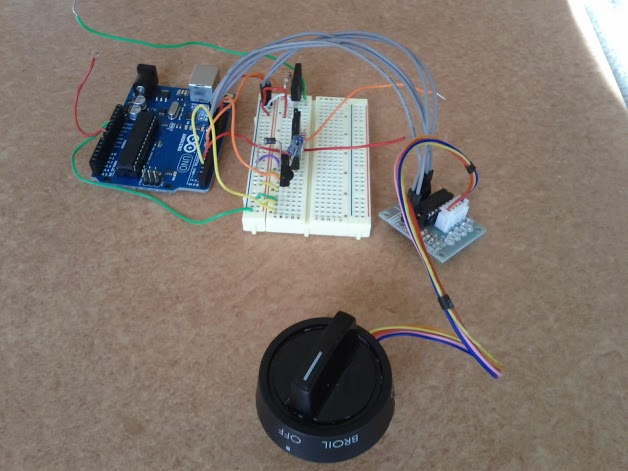
\includegraphics[width=\linewidth]{vendos.png}
  \caption{Arduino connected to oven controlling stepper motor}
  \label{fig:marginparsample}
  \end{center}  
\end{figure}


We would like the system to be able to integrate with all kinds of appliances the user already owns without having to purchase specialized equipment or requiring to substantially alter the circuitry or design of the appliance.
We would also like to give the user more control than simply powering on or off the appliance.

We have 4 different kind of outputs to control external appliances.
\begin{itemize}\compresslist
\item
Relay
\item
Regulator
\item
Infrared Emitter
\item
Stepper motor
\end{itemize}


An Arduino Uno Rev. 3  has 14 digital I/O ports six of which can produce pulse-width modulated signals (can be rapidly turned on and off at a certain frequency), and six analog (ON or OFF state) inputs.
Each kind of output need a certain number and type of these ports uniquely mapped for each (unless the user would like for a I/O port to control more than one output at all times) as well as have a different function and way to control the appliance.
However, the user can easily extend the number of ports to control virtually an unlimited number of appliances in the home. \cite{_arduino}

\subsection{Relay}
The most basic way to control an appliance is to turn it on or off.
Using a solid state relay, the circuit acts like a computer-controlled wall-switch.
It requires 1 I/O port (analog or PWM) and our version can switch up to 240VAC 8A loads. \cite{_control}

\begin{figure}
  \begin{center}
  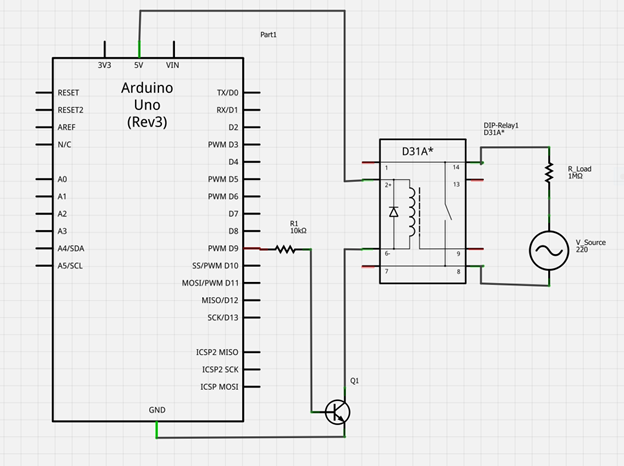
\includegraphics[width=\linewidth]{schematic.png}
  \caption{Arduino relay schematic}
  \label{fig:relay}
  \end{center}  
\end{figure}

\subsection{Regulator}
Many people would like the flexibility to adjust the brightness of a light bulb, speed of a motor, or level of a speaker without simply just turning them on or off.
The dimmer circuit uses a simple MOSFET like a switch to control a DC circuit.
Lowering the frequency will cause the circuit to be on less frequently, which will cause light bulbs to dim and motors to slow down and vice versa. 
It uses 1 PWM I/O port to control the MOSFET and can handle switching up to 60V, and the amperage is limited to 30A. \cite{_bildr}

\begin{figure}
  \begin{center}
  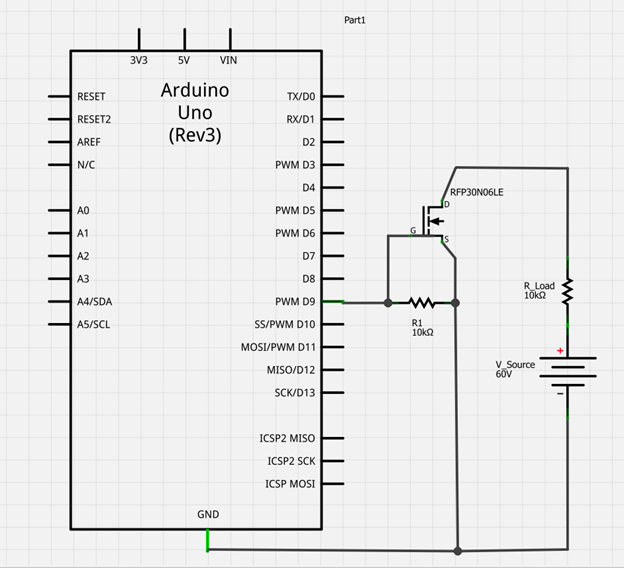
\includegraphics[width=\linewidth]{schematic_2.png}
  \caption{Arduino regulator schematic}
  \label{fig:regulator}
  \end{center}  
\end{figure}


In this iteration, we used the circuit to control an LED light bulb

\subsection{Infrared Emitter}
Many appliances, such as TV and DVD players, utilize Infrared (IR) light to communicate with other devices, namely remote controls.
The Arduino can also act like a remote control with an IR LED attached to 1 PWM I/O port.
Additionally, an IR LED Receiver, attached to 1 analog I/O port, can open opportunities to do two-way communication with the appliance and Arduino. \cite{_how_to_tv}

In this iteration, we used a RadioShack High-Powered Infrared LED with a radiant power output of 16mW minimum for the emitter and an IR LED Receiver to record the Apex LE2612D TV remote control encodings for power on/off, volume up, volume down, channel up, channel down, and inputting a specific channel. 

\subsection{Stepper motor}
There are some appliances that cannot be simply directly wired, like opening curtains or preheating the oven to specific temperatures.
Stepper motors fill the void of where precise human interaction is required.
With proper setup, the stepper motor can be used for simple actions such as turning, pushing, and pulling which can be utilized for more complex actions like turning an over knob.
It requires 3 PWM and 1 analog I/O ports. \cite{_how_to_motors}

In this iteration, we attached a stepper motor to a disconnected oven knob to specific degrees (375, 400, 425, 450, and 475 degrees Fahrenheit). 

% =============================================================================

% =============================================================================
\section{Evaluation (Software)}
% =============================================================================

The current implementation of Vendos works to satisfaction, but limits of the Kinect such as field of vision impair the accuracy of some gesture detection.
Voice detection also tends to be too sensitive, catching background noise and not processing commands accurately.
 
Some current gestures, such as “Swipe Down” and gestures involving multiple body parts are more troublesome to detect than others, perhaps in future implementations, better gestures can be decided upon and implemented.

% =============================================================================
\section{Evaluation (Hardware)}
% =============================================================================


Due to time constraints, we were unable to test and benchmark the relay circuit.
However, we expect that it should be function and very easy to debug since there are only 2 kinds of inputs and 2 kinds of output (ON or OFF).
One possible challenge with this method is that it is wired; if the user wanted to control an appliance from a long distance (e.x. on the other side of a bedroom), then they would have to connect a correspondingly-lengthened wire from the Arduino to the appliance, which could be cumbersome and intrusive for the user to install.

The regulator circuit worked satisfactorily as the LED light bulb brightened all the way to the brightest it can be as well as dimmed all the way to being turned off on command.
Unfortunately, one limitation with our implementation is that it only works with DC loads, which disallows this circuit to be used with room lights and common household lamps.
Additionally, it is wired, which has its share of problems as stated above.
In future iterations, we will try using a solid state relay with an optically isolated Triac as a regulator circuit \cite{_arduino_lights}.

The infrared emitter worked as intended but with a severe limitation;
it had to placed about 5 inches in front of the television's IR detector for it to work.
We suspect that using an IR LED with a radiant power output should be able to reach detectors from a much longer distances.
Additionally, for the TV itself, there must be a considerable delay (about 5 seconds) in-between different commands, otherwise the TV would incorrectly execute another command.
However, the proof-of-concept now exists and this opens up the possibilities to use IR switches as remote relays for appliances.
Although infrared relieves the need to and difficulty of install long wirings, it has its own design considerations;
the IR emitter and detector must have a clear line-of-sight from each other so the emitter should be installed in the top corner of a room and all detectors must be exposed and not be blocked by the environment, which could be more troublesome than directly wiring in some cases.

The stepper motor precisely turned the knob to the specified degree precisely.
However, because it was disconnected from the oven, it faced less torque resistance.
In future iterations, a proper mount and, possibly, transmission box should be connected to between the stepper motor and the attached oven knob.
Additionally, we were unable to test pulling and pushing action, but in theory, such actions can be done with a pulley system.

% =============================================================================
\section{Discussion}
% =============================================================================

Through multiple iterations of Vendos were also able to gather valuable feedback about using commonly sourced and cost-efficient consumer products to build a home automation device.
We built our product around three main points: cost-effectiveness, integration, and usability.
 
Our main focus is to be cost effective.
Although there are already home automation solutions built for the Kinect, it relied on expensive automation controllers that cost \$575 \cite{_nitrogen} just for the adapters.
In addition, as our primary target audience is towards the elderly, most of the features implemented in those automation controllers are unnecessary.
Thus, we chose to focus on just core components of objects in an elderly home: lights, television and appliances.
By building around such objects, we were able to buy consumer parts and built a very cost efficient prototype.
Not including the cost of the Arduino and the Kinect, the price of other parts totaled only \$15.86.

While this price is how much we spent buying the parts individually as consumers, if mass-produced the price would go down as well.
For example, at the time of writing this paper, the stepper motor we purchased costs \$5.12 but if we purchased with bulk quantity and pricing, it would be as low as \$0.10 per stepper motor \cite{_stepper_motor}.
By using open source technologies such as Arduino \cite{_arduino_policy}, we are able to keep the cost down, even with future implementations of more features to simplify use.
 
We integrated basic functions for television, appliances and lights through the Arduino.
We change degrees of brightness through Kinect sending the Arduino multiple pulse width modulation (PwM) levels, we provide appliance control through a stepper motor (such as for turning on/off oven), and we are able to control channels of the television with an IR Emitter.

For an elderly home, those are the main sources of daily usage. We designed this project to be modular as each individual example is a template for multiple custom device designs.
The same template used to control lights can be used to control any AC wall outlet devices that have multiple levels of intensities, such as fans, or even Christmas lights for decoration.
The design for an oven knob control has a base of a stepper motor, which can also be used to move curtains and can be a base template of any contraption that requires motion movement.
In addition, with the implementation of gesture and voice recognition, having an emphasis on the safety of the elderly user is paramount.
Regardless of how simple an automated home is, they might still be prone to accidents. 

In the future, we would like to implement motion detection for safety as well.
For example, if an elderly person has fallen the Kinect can detect such movements and instantly call an emergency number.
Using multiple Kinect devices and using KinectFusion \cite{_kinect_fusion} to construct a composite 3D model of the user's entire skeleton from multiple angles could be useful to build a model accurate enough for this kind of application.
At the moment however, KinectFusion requires lots of processing power and would require increases in speed spread over many low power devices or a single high powered machine in the home. 

In addition, with the release of Kinect 2 there are already multiple improvements that has been built into the device that can improve support of the elderly.
Currently the Kinect 2 has an IR blaster and the Xbox One already has an implementation of Universal TV Control \cite{_control_tv}.
There are also applications for the Kinect 2 that provide heart rate monitoring \cite{_xbox_fitness}, a feature that could prove useful in irregular heartbeat detection (heart attacks).
We see this as evidence that the Kinect has a strong role to play in body and health monitoring in the home.

At the moment, our Vendos proof of concept for the accessibility of light and appliance movement is still limited to being physically connected to the Arduino itself, creating a possible safety hazard for inattentive users.
However, with the consumer adaptation of Low-Powered Bluetooth and WiFi Direct, it might be possible to implement house features using those designs.
Currently a company called Lockitron has already implemented a door locking device that attaches onto any deadbolt, and is controlled through WiFi and Bluetooth by a mobile phone application\cite{_lockitron}.
Such system provides a working example of adding features to an already working home, proving that it is possible to integrate automation tools into any home.
With the new release of Arduino Yun, which is an Arduino with wireless interface \cite{_arduino_yun}, it is possible to migrate our current setup of home automation to being wirelessly connected.
In addition, a wireless interface will still provide modularity in adapting home automation tools as the interaction hardware themselves aren't changed. 

From a usability point of view, we are able to utilize commonly used gestures and provide voice commands that are easy to remember and use.
However, due to the inaccuracy of the Kinect, there has been mistakes in reading the gestures and voice listening.
Fortunately, as the camera in the Kinect has a very low resolution, Kinect 2 should fixed these shortcoming as both the microphone and camera have been upgraded and will provide more accurate usability.
We would also like to build an application for users to program their own voice and gesture commands to do such actions as that will provide elderly with more options on how to define their actions and voice.

% =============================================================================
\section{Conclusion}
% =============================================================================

We demonstrated how voice controls and gestures obtained from low cost commodity hardware can be successfully integrated into a home automation solution.
The accuracy of controls is not yet at an acceptable point where such a system could be relied upon solely for taking care of common household tasks.
Despite the flaws in current voice and gesture recognition systems, our solution has value to the common person and people who are mostly independent.
The lack of physical controls used in our approach has interesting implications on how normal households have formed their workflows.
In a future where your house may be able to talk back to you and hear all of your commands, we will see the quality of all our lives increase.

However, our solution will need to grow beyond the limitations of current speech recognition abilities and gesture interpretation.
For a system that may be relied upon to save lives, any mistakes could result in lives lost.
At this stage, Vendos deployed in a real nursing home would probably be too frustrating for caretakers and users alike to deal with.
Our outlook on this project is still optimistic and the hardware necessary to integrate it into real homes is on track to grow stronger and cheaper.

\section{Acknowledgements}

We thank our professor, Dr. Nadir Weibel, for organizing CSE 118 - Ubiquitous Computing at the University of California, San Diego and providing materials needed to complete this project.
We also thank our TA, Eric Seidel, for offering his assistance in discussion with setting up the Kinect for Windows SDK, constructing presentations, and writing this paper.

\balance
\bibliographystyle{acm-sigchi}
\bibliography{references}

\end{document}
